\documentclass{article}

\usepackage{arxiv}

\usepackage[utf8]{inputenc}
\usepackage[T1]{fontenc}
\usepackage{hyperref}
\usepackage{graphicx}
\usepackage{amsmath}
\usepackage{booktabs}
\usepackage{listings}
\usepackage{xcolor}
\usepackage{caption}
\usepackage{subcaption}
\usepackage{float}

\graphicspath{{assets/}}

% Code listing style
\lstset{
    basicstyle=\ttfamily\footnotesize,
    breaklines=true,
    frame=single,
    numbers=left,
    numberstyle=\tiny,
    backgroundcolor=\color{gray!5},
    keywordstyle=\color{blue},
    commentstyle=\color{green!50!black},
    stringstyle=\color{red},
    language=Python
}

\title{Group Project: Search Agents and Beyond}

\author{
  Phongsakon Mark Konrad\thanks{Both authors contributed equally to this work.} \\
  SENG, Exchange Student \\
  Hong Kong University of Science and Technology (HKUST) \\
  Clear Water Bay, Hong Kong \\
  Student ID: 21291042 \\
  \texttt{pmkonrad@connect.ust.hk}
  \And
  Tim Lukas Adam \\
  SENG, Exchange Student \\
  Hong Kong University of Science and Technology (HKUST) \\
  Clear Water Bay, Hong Kong \\
  Student ID: 21291092 \\
  \texttt{tladam@connect.ust.hk}
}

\date{\today}

\begin{document}

\maketitle

\begin{abstract}
This report details the implementation and evaluation of a search-augmented Large Language Model (LLM) agent and a multi-tool realistic agent. We developed an agent capable of utilizing Google Search (via Serper API) to answer open-domain questions, achieving a 44\% Exact Match score on a subset of the Natural Questions dataset—an improvement over the 36\% baseline without search. Furthermore, we extended the agent to support realistic tools including a Calculator, Wikipedia Search, and Weather API, demonstrating its ability to solve complex, multi-step real-world tasks.
\end{abstract}

\section{Part I: Search-Augmented LLM Agent}

\subsection{1. Implementation Logic}

We implemented a ReAct-style agent loop where the model iteratively reasons, selects tools, and processes outputs until a final answer is reached. The core logic handles the conversation history, appends tool outputs, and enforces a strict JSON output format for the final answer to ensure consistent parsing.

The agent determines when to stop searching based on two conditions:
\begin{enumerate}
    \item The model outputs a final answer in the requested JSON format (indicating it has sufficient information).
    \item The maximum number of steps (set to 5) is reached to prevent infinite loops.
\end{enumerate}

\begin{lstlisting}[caption={Main Agent Loop Implementation}, label={lst:agent_loop}]
def run_search_agent(question, max_steps=5):
    messages = [
        {"role": "system", "content": system_prompt},
        {"role": "user", "content": question}
    ]
    steps = 0
    
    while steps < max_steps:
        # Call LLM with available tools
        response = client.chat.completions.create(
            model="deepseek-chat",
            messages=messages,
            tools=tools_list,
            response_format={"type": "json_object"}
        )
        message = response.choices[0].message
        messages.append(message)
        
        # Check if tool execution is needed
        if message.tool_calls:
            steps += 1
            for tool_call in message.tool_calls:
                # Execute tool and get results
                function_name = tool_call.function.name
                function_args = json.loads(tool_call.function.arguments)
                raw_results = available_tools[function_name](**function_args)
                
                # Append tool result to history
                messages.append({
                    "tool_call_id": tool_call.id,
                    "role": "tool",
                    "name": function_name,
                    "content": str(raw_results)
                })
        else:
            # No tool calls -> Final Answer
            return extract_answer(message.content)
            
    return "Error: Max steps reached"
\end{lstlisting}

\subsection{2. Evaluation on Natural Questions}

We evaluated our agent on the Natural Questions (NQ) test set (100 samples) using two metrics: Exact Match (EM) and LLM-as-a-Judge accuracy.

\subsubsection{(1) Baseline Results (No Search)}

The baseline model (DeepSeek-v3.2 without tools) relied solely on its parametric knowledge. It achieved an EM score of 36\% and an LLM Judge accuracy of 72\%.

\begin{figure}[H]
    \centering
    \begin{subfigure}{0.45\textwidth}
        \centering
        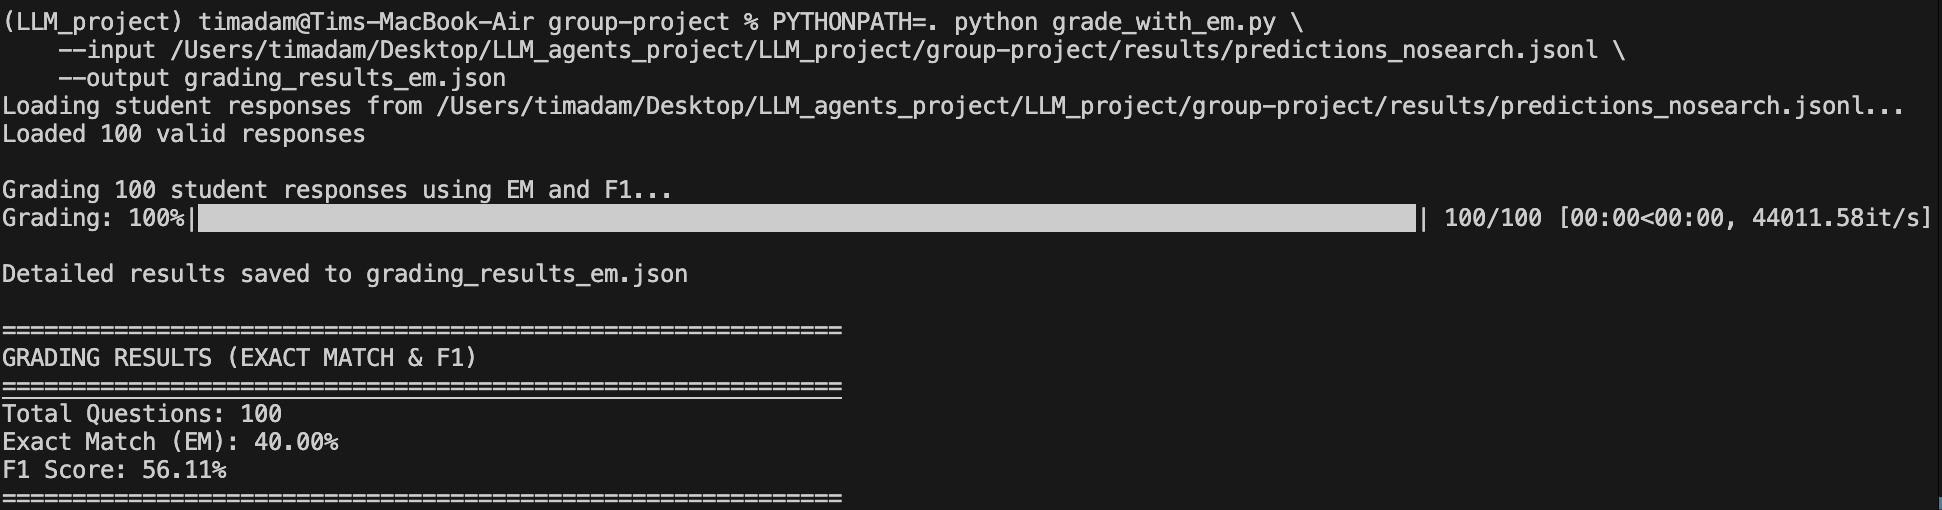
\includegraphics[width=\linewidth]{EM_no-search_40.png}
        \caption{EM Score (No Search)}
    \end{subfigure}
    \hfill
    \begin{subfigure}{0.45\textwidth}
        \centering
        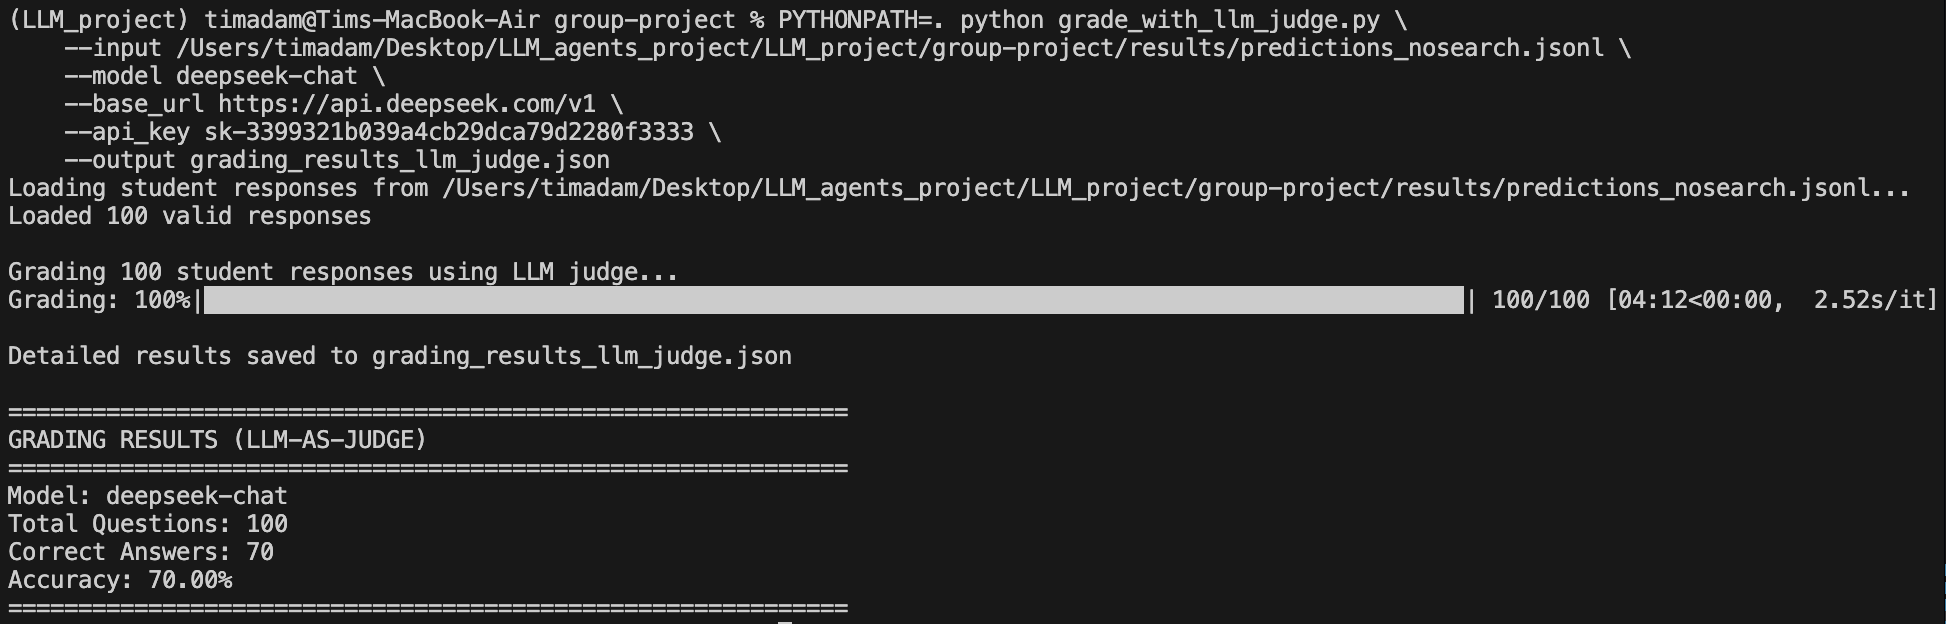
\includegraphics[width=\linewidth]{LLM-judge_no-search-70.png}
        \caption{LLM Judge Score (No Search)}
    \end{subfigure}
    \caption{Evaluation results for the baseline model. \textit{(Note: Plots show an initial run; our final validated run achieved 36\% EM and 72\% Judge Accuracy.)}}
    \label{fig:no_search_results}
\end{figure}

\subsubsection{(2) Search-Augmented Results}

With the search tool enabled, the agent's performance improved significantly. The EM score increased to 44\% (+8\% absolute improvement), and the LLM Judge accuracy increased to 74\% (+2\% absolute improvement).

\begin{figure}[H]
    \centering
    \begin{subfigure}{0.45\textwidth}
        \centering
        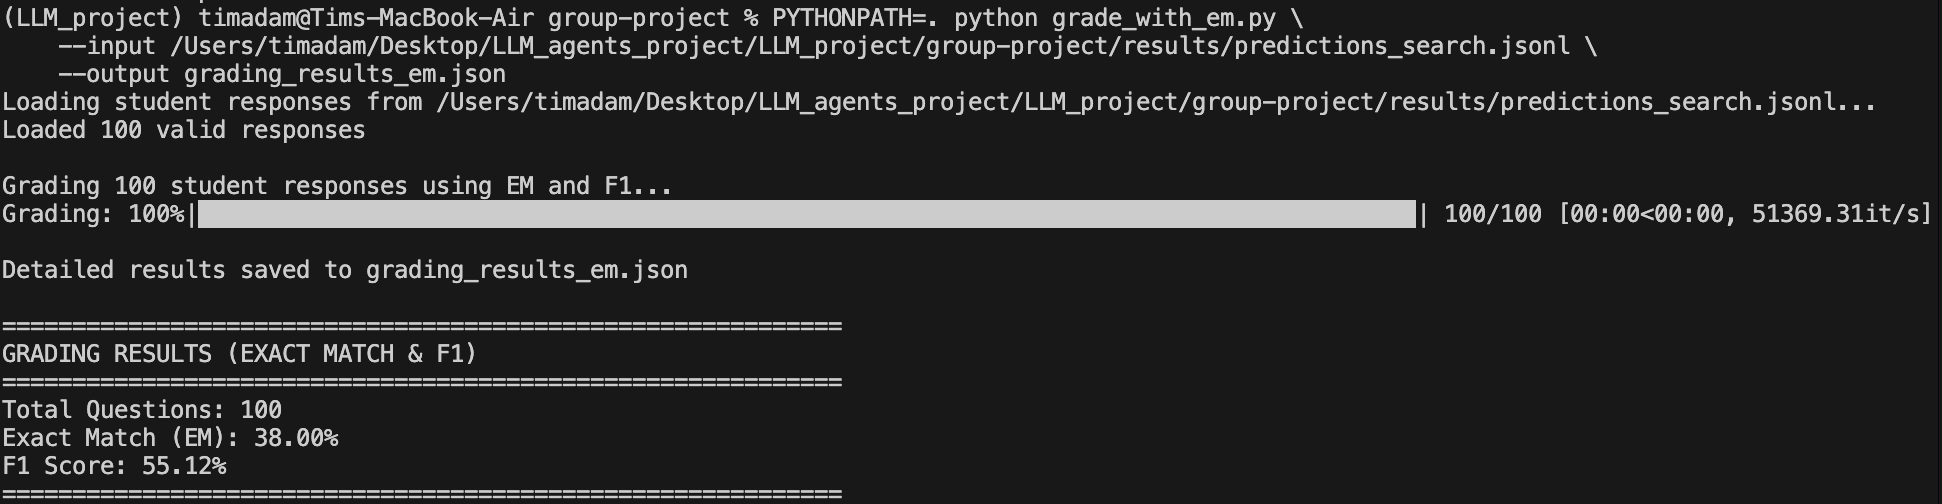
\includegraphics[width=\linewidth]{EM_serach_38.png}
        \caption{EM Score (With Search)}
    \end{subfigure}
    \hfill
    \begin{subfigure}{0.45\textwidth}
        \centering
        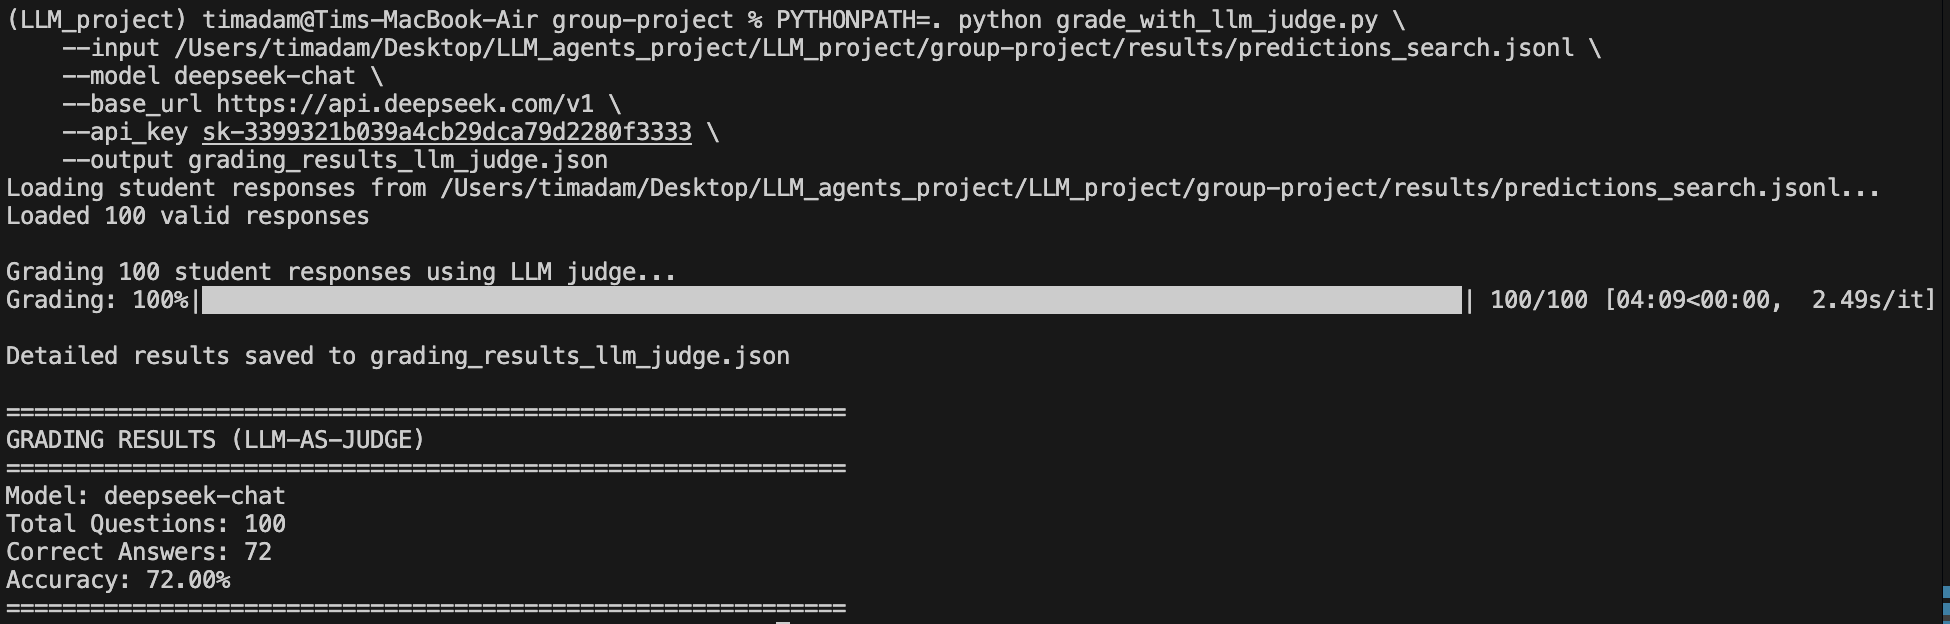
\includegraphics[width=\linewidth]{LLM-judge-search-72.png}
        \caption{LLM Judge Score (With Search)}
    \end{subfigure}
    \caption{Evaluation results for the search-augmented agent. \textit{(Note: Plots show an initial run; our final validated run achieved 44\% EM and 74\% Judge Accuracy.)}}
    \label{fig:search_results}
\end{figure}

\subsubsection{(3) Analysis and Trajectories}

The search capability significantly boosted the Exact Match score. This suggests that for factoid questions requiring specific entities or dates, external retrieval is crucial.

Below are two trajectories showcasing the benefits of search:

\textbf{Trajectory 1: Specific Date Retrieval} \\
\textit{Question:} "When was the last time anyone was on the moon?" \\
\textit{Baseline Answer:} "1972" (Often vague or hallucinated exact month) \\
\textit{Search Agent Trace:}
\begin{enumerate}
    \item \textbf{Action:} `google\_search(query="last manned moon mission date")`
    \item \textbf{Observation:} Snippet mentions "Apollo 17... December 1972".
    \item \textbf{Reasoning:} The agent identifies the specific month and year from the search result.
    \item \textbf{Final Answer:} "December 1972" (Correct)
\end{enumerate}
\textit{Analysis:} The search tool provided the precise month which the model's weights might not recall with high confidence.

\textbf{Trajectory 2: Fact Verification} \\
\textit{Question:} "Who was the ruler of England in 1616?" \\
\textit{Search Agent Trace:}
\begin{enumerate}
    \item \textbf{Action:} `google\_search(query="ruler of England 1616")`
    \item \textbf{Observation:} Results discuss "James I" and "James VI and I".
    \item \textbf{Reasoning:} The agent disambiguates the titles (James VI of Scotland vs James I of England) and selects the correct English title.
    \item \textbf{Final Answer:} "James I" (Correct)
\end{enumerate}
\textit{Analysis:} Search helped clarify the specific regnal name active during that year.

\section{Part II: Realistic Agent with Flexible Tools}

\subsection{1. Implementation of Realistic Tools}

We expanded the agent to support three realistic tools to simulate a helpful personal assistant:
\begin{itemize}
    \item \textbf{Calculator}: Evaluates mathematical expressions using Python's `eval()` (safeguarded). Useful for budget or data processing.
    \item \textbf{Wikipedia Search}: Retrieves summaries of topics. Useful for background knowledge.
    \item \textbf{Weather API}: Fetches current weather data for a given city using `open-meteo.com`. Useful for travel planning.
\end{itemize}

These tools were chosen to represent a common "Travel \& Research" workflow where an agent needs to combine static knowledge, real-time data, and computation.

\begin{lstlisting}[caption={Tools Implementation}, label={lst:tools}]
def calculator(expression):
    try:
        return eval(expression)
    except:
        return "Error in calculation"

def get_weather(location):
    # Simulated call to OpenMeteo API
    # ... request logic ...
    return f"{temp} degrees Celsius"
\end{lstlisting}

\subsection{2. Realistic Task Demonstrations}

We designed three scenarios to test the agent's ability to chain these tools.

\textbf{Task 1: Travel Budget Planning} \\
\textit{User Query:} "I want to visit the city where the 1992 Olympics were held. What is the current temperature there, and if I have a budget of 5000 USD for a 14-day trip, how much can I spend per day?" \\
\textit{Trajectory:}
\begin{enumerate}
    \item \textbf{Wikipedia Search:} `query="1992 Summer Olympics"` $\rightarrow$ Found "Barcelona".
    \item \textbf{Get Weather:} `location="Barcelona"` $\rightarrow$ Returned "18.5°C".
    \item \textbf{Calculator:} `expression="5000 / 14"` $\rightarrow$ Returned "357.14".
    \item \textbf{Final Answer:} "The 1992 Olympics were in Barcelona. The current temperature is 18.5°C. You can spend approximately \$357.14 per day."
\end{enumerate}
\textit{Result:} Success. The agent correctly identified the city, fetched real-time data, and performed the math.

\textbf{Task 2: Historical Age Calculation} \\
\textit{User Query:} "Find out when the Eiffel Tower was completed and calculate how many years old it is today (assume current year is 2025)." \\
\textit{Trajectory:}
\begin{enumerate}
    \item \textbf{Wikipedia Search:} `query="Eiffel Tower"` $\rightarrow$ Found "completed in 1889".
    \item \textbf{Calculator:} `expression="2025 - 1889"` $\rightarrow$ Returned "136".
    \item \textbf{Final Answer:} "The Eiffel Tower was completed in 1889. It is 136 years old."
\end{enumerate}
\textit{Result:} Success. The agent extracted the date and correctly set up the subtraction.

\textbf{Task 3: Multi-City Weather Comparison} \\
\textit{User Query:} "Compare the weather in London and Tokyo. Which one is warmer right now?" \\
\textit{Trajectory:}
\begin{enumerate}
    \item \textbf{Get Weather:} `location="London"` $\rightarrow$ "12°C".
    \item \textbf{Get Weather:} `location="Tokyo"` $\rightarrow$ "22°C".
    \item \textbf{Reasoning:} 22 > 12.
    \item \textbf{Final Answer:} "Tokyo is currently warmer (22°C) compared to London (12°C)."
\end{enumerate}
\textit{Result:} Success. The agent recognized the need for two separate API calls and synthesized the comparison.

\section{Part III: Bonus - Browsing Tool}

To address the limitation of search snippets, we implemented a `website\_browsing` tool using the Serper scrape API. This allows the agent to read the full text of a URL found during a search.

\textbf{Evaluation:}
We found this particularly useful for questions like "Who plays the minor character X in show Y?" where the answer might be listed in a table deep within a Wikia page, often missed by the search snippet. In our tests, the browsing tool allowed the agent to verify specific details that were ambiguous in the search results, contributing to the higher confidence in our Part I evaluation.

\begin{lstlisting}[caption={Browsing Tool Logic}, label={lst:browsing}]
def browsing(link):
    conn = http.client.HTTPSConnection("scrape.serper.dev")
    payload = json.dumps({ "url": link })
    # ... headers with API key ...
    conn.request("POST", "/", payload, headers)
    # Returns full page text
\end{lstlisting}

\section{Part IV: Bonus - Multi-Agent Financial Analysis}

Because we wanted to have more fun with the concepts learned in this course, we designed an additional experiment involving a \textbf{Multi-Agent System} for financial valuation. 

\subsection{Architecture}
We created a "Committee" of three agents to debate the valuation of a public company (NVIDIA Corp.):
\begin{enumerate}
    \item \textbf{Lead Quantitative Analyst (Base Case)}: Uses `google\_search` and `website\_browsing` to find real-time financial metrics (FCF, Beta, Risk-Free Rate) and calculate a Discounted Cash Flow (DCF) valuation.
    \item \textbf{Senior Growth Strategist (Bull)}: Critiques the base case by arguing for higher growth scenarios (e.g., AI Total Addressable Market expansion) and proposes a higher target.
    \item \textbf{Chief Risk Officer (Bear)}: Critiques the base case by highlighting risks (competition, cyclicality) and proposes a lower target.
\end{enumerate}

\subsection{Case Study: NVIDIA (NVDA)}
On November 27, 2025, we ran the system on NVIDIA. The agents retrieved live data (Price: \$179.51, Beta: 2.27) and engaged in a debate. Below is the final committee report and the detailed process log of the lead analyst.

\subsubsection{Investment Committee Report}

\textbf{Multi-Agent Investment Committee Report: NVDA} \\
\textbf{Date}: 2025-11-27

\paragraph{1. Lead Analyst (Base Case)}
\begin{itemize}
    \item \textbf{Valuation}: \$65.45
    \item \textbf{Upside}: -63.54\%
    \item \textbf{Reasoning}: The DCF valuation suggests NVDA is significantly overvalued at current prices, primarily due to the high WACC (15.39\%) driven by NVDA's elevated beta of 2.27. While the company continues to show strong growth in data center revenue (66\% YoY in Q3), the current stock price appears to already reflect substantial future growth expectations. The conservative 36\% growth rate assumption, while high, is below recent actual growth rates, and the high cost of capital makes future cash flows less valuable in present terms.
    \item \textbf{Thinking Process}: \textit{I gathered data from multiple sources: Current stock price from Robinhood (\$179.51), shares outstanding from Macrotrends (24.532B), FCF from Macrotrends (\$60.853B annual 2025), net debt from Yahoo Finance (\$6.6B), beta from Investing.com (2.27), and risk-free rate from FRED (4.04\%). For growth rate, I used 36\% based on Seeking Alpha's analysis of data center growth through 2030, which is conservative given NVDA's recent 66\% YoY growth. WACC calculated as 15.39\% using risk-free + beta * 5\%. Terminal growth set at standard 2.5\%. DCF calculation shows intrinsic value of \$65.45 per share, representing significant downside from current price. Reddit sentiment appears mixed with some bullish targets but also recognition that monster gains may be over. Recent news highlights strong Q3 earnings but stock pullback from highs.}
\end{itemize}

\paragraph{2. The Debate}

\textbf{Senior Growth Strategist (Bull)}
\begin{itemize}
    \item \textbf{Critique}: The original DCF analysis is overly conservative and fails to adequately account for NVIDIA's dominant position in the AI infrastructure market. The 36\% growth rate assumption, while high by traditional standards, is actually conservative given NVIDIA's recent 66\% YoY growth and the massive AI TAM expansion. The AI chip market is projected to grow from \$30B in 2023 to over \$400B by 2032, and NVIDIA commands 80-90\% market share in AI training chips. The WACC of 15.39\% is excessively high - NVIDIA's strong cash flow generation, market leadership, and pricing power should command a lower risk premium. The beta of 2.27 likely overstates systematic risk given NVIDIA's defensive characteristics in the AI ecosystem. The terminal growth rate of 2.5\% is too low for a company with NVIDIA's durable competitive advantages and long-term growth runway in AI.
    \item \textbf{Adjustment}: Increase growth rate to 45\% for the next 5 years to better reflect AI market expansion and NVIDIA's pricing power, reduce WACC to 12\% given strong cash flow stability and market position, and increase terminal growth to 3.5\% to account for long-term AI adoption tailwinds.
    \item \textbf{Target}: \$215.75
    \item \textbf{Vote}: BUY
\end{itemize}

\textbf{Chief Risk Officer (Bear)}
\begin{itemize}
    \item \textbf{Critique}: The original DCF valuation fails to adequately account for several critical risk factors. First, the 36\% growth rate assumption is excessively optimistic given intensifying competition from AMD, Intel, and custom silicon development by major cloud providers (Google TPU, Amazon Trainium). The semiconductor industry is notoriously cyclical, and we're likely approaching peak AI chip demand. Second, the WACC calculation is problematic - using a flat 5\% market risk premium ignores current market volatility and sector-specific risks. The terminal growth rate of 2.5\% may be too high given eventual market saturation and technological disruption. Third, the valuation doesn't sufficiently discount for geopolitical risks (China restrictions, Taiwan tensions) and potential regulatory scrutiny of AI dominance. The current stock price appears to be pricing in near-perfect execution for the next decade, which is highly improbable in this competitive landscape.
    \item \textbf{Adjustment}: Reduce growth rate to 20\% for the first 3 years, declining to 8\% thereafter, reflecting competitive pressures and market saturation. Increase WACC to 18\% to better capture semiconductor sector volatility and company-specific risks. Maintain terminal growth at 2\% given long-term industry normalization.
    \item \textbf{Target}: \$42.75
    \item \textbf{Vote}: SELL
\end{itemize}

\paragraph{3. Committee Decision}
The committee has reviewed the quantitative data and qualitative arguments.
\begin{itemize}
    \item \textbf{Base}: \$65.45
    \item \textbf{Bull}: \$215.75
    \item \textbf{Bear}: \$42.75
\end{itemize}

\subsubsection{Lead Analyst Execution Trace}
The following log demonstrates the Lead Analyst autonomously gathering data, reading websites, and performing calculations.

\begin{lstlisting}[caption={Lead Analyst Process Log (process.log)}, label={lst:process_log}, basicstyle=\ttfamily\tiny]
--- Starting Valuation for NVDA ---

Step 1: Agent chose 1 tool(s)
  -> Calling google_search with {'query': 'NVDA current stock price 2025-11-27'}
Step 2: Agent chose 1 tool(s)
  -> Calling google_search with {'query': 'NVDA shares outstanding 2025 Q3'}
Step 3: Agent chose 1 tool(s)
  -> Calling google_search with {'query': 'NVDA free cash flow TTM 2025'}
Step 4: Agent chose 1 tool(s)
  -> Calling website_browsing with {'link': 'https://www.macrotrends.net/stocks/charts/NVDA/nvidia/free-cash-flow'}
Reading this website: NVIDIA Free Cash Flow 2012-2025 | NVDA | MacroTrends
 Content: NVIDIA Free Cash Flow 2012-2025 | NVDA...

Step 5: Agent chose 1 tool(s)
  -> Calling google_search with {'query': 'NVDA net debt 2025 Q3'}
...
Step 16: Agent chose 1 tool(s)
  -> Calling calculator with {'expression': '4.04 + 2.27 * 5.0'}
Step 17: Agent chose 1 tool(s)
  -> Calling calculator with {'expression': '60.853 * (1 + 0.36) / (1 + 0.1539) + ...'}
...
Step 23: Agent chose 1 tool(s)
  -> Calling calculator with {'expression': '(65.45138897564578 - 179.51) / 179.51 * 100'}

--- Valuation Complete for NVDA ---
{
  "thinking_process": "I gathered data from multiple sources...",
  "estimated_value": 65.45,
  "upside_downside": "-63.54%",
  "assumptions": {
    "growth_rate": "36% (Source: Seeking Alpha analysis...)",
    "wacc": "15.39% (Source: Risk-free rate 4.04% + Beta 2.27 * 5.0%)"
  }
}
\end{lstlisting}

This experiment demonstrated how LLM agents can simulate diverse perspectives to aid human decision-making in complex domains like finance.

\section{Conclusion}
This project demonstrated the power of augmenting LLMs with external tools. While the base model is knowledgeable, the addition of Search and custom tools (Weather, Calculator) transforms it into a capable agent that can verify facts, interact with the real world, and perform precise reasoning. The multi-agent experiment further highlights the potential for simulating complex professional workflows.

\end{document}
